\printconcepts

\exercise{T/F: The Product Rule states that $\ds \frac{\dd}{\dd x}\big(x^2\sin x\big) = 2x\cos x$.}{F}

\exercise{T/F: The Quotient Rule states that $\ds \frac{\dd}{\dd x}\left(\frac{x^2}{\sin x}\right) = \frac{2x}{\cos x}$.}{F}

\exercise{T/F: The derivatives of the trigonometric functions that start with ``c'' have minus signs in them.}{T}

\exercise{What derivative rule is used to extend the Power Rule to include negative integer exponents?}{Quotient Rule}

\exercise{T/F: Regardless of the function, there is always exactly one right way of computing its derivative.}{F}

\exercise{In your own words, explain what it means to make your answers ``clear.''}{Answers will vary.}

%\exercise{Give an example of a function where $\fp(x) \neq 0$ and $\fpp(x) = 0$.}{One possible answer is $f(x) = 17x-205$.}

%\exercise{Explain in  your own words what the second derivative ``means.''}{Answers will vary.}

%\exercise{If $f(x)$ describes a position function, then $\fp(x)$ describes what kind of function? What kind of function is $\fpp(x)$?}{$\fp(x)$ is a velocity function, and $\fpp(x)$ is acceleration.}

%\exercise{Let $f(x)$ be a function measured in pounds, where $x$ is measured in feet. What are the units of $\fpp(x)$?}{lbs/ft$^2$.}

\printproblems

\exercisesetinstructions{, use the Quotient Rule to verify these derivatives.}

\exercise{$\dfrac{\dd}{\dd x}(\cot x) = -\csc^2 x$}{\mbox{}\\[-2\baselineskip]\parbox[t]{\linewidth}{\begin{align*}
\frac{\dd}{\dd x}(\cot x)
&=\frac{\dd}{\dd x}\left(\frac{\cos x}{\sin x}\right)\\
&=\frac{\sin x (-\sin x) - (\cos x)(\cos x)}{(\sin x)^2}\\
&=\frac{-[(\sin x)^2 + (\cos x)^2]}{(\sin x)^2}\\
&=\frac{-1}{(\sin x)^2} = -\csc^2 x
\end{align*}}}

% cut for parity
%\exercise{$\dfrac{\dd}{\dd x}(\sec x) = \sec x \tan x$}{\mbox{}\\[-2\baselineskip]\begin{align*}
%\frac{\dd}{\dd x}(\sec x)
%&=\frac{\dd}{\dd x}\left(\frac{1}{\cos x}\right)\\
%&=\frac{\cos x \cdot 0 - 1 \cdot (-\sin x)}{(\cos x)^2}\\
%&=\frac{\sin x}{(\cos x)^2} = \sec x \tan x
%\end{align*}}

\exercise{$\dfrac{\dd}{\dd x}(\csc x) = -\csc x \cot x$}{\mbox{}\\[-2\baselineskip]\parbox[t]{\linewidth}{\begin{align*}
\frac{\dd}{\dd x}(\csc x)
&=\frac{\dd}{\dd x}\left(\frac{1}{\sin x}\right)\\
&=\frac{\sin x \cdot 0 - 1 \cdot (\cos x)}{(\sin x)^2}\\
&=\frac{-\cos x}{(\sin x)^2} = -\csc x \cot x
\end{align*}}}

\exercisesetend


\begin{exerciseset}{In Exercises}{:
\begin{enumerate}
\item Use the Product Rule to differentiate the function.
\item Manipulate the function algebraically and differentiate without the Product Rule.
\item Show that the answers from (a) and (b) are equivalent.
\end{enumerate}}

\exercise{$f(x) = x(x^2+3x)$}{\mbox{}\\[-2\baselineskip]\parbox[t]{\linewidth}{\begin{enumerate}
\item $\fp(x) = (x^2+3x) + x(2x+3)$
\item $\fp(x) = 3x^2 + 6x$
\item They are equal.
\end{enumerate}}}

\exercise{$g(x) = 2x^2(5x^3)$}{\mbox{}\\[-2\baselineskip]\parbox[t]{\linewidth}{\begin{enumerate}
\item $g'(x) = 4x(5x^3)+2x^2(15x^2)$
\item $g'(x) = 50x^4$
\item They are equal.
\end{enumerate}}}

\exercise{$h(s) = (2s-1)(s+4)$}{\mbox{}\\[-2\baselineskip]\parbox[t]{\linewidth}{\begin{enumerate}
\item $h'(s) = 2(s+4) + (2s-1)(1)$
\item $h'(s) = 4s + 7$
\item They are equal.
\end{enumerate}}}

\exercise{$f(x)= (x^2+5)(3-x^3)$}{\mbox{}\\[-2\baselineskip]\parbox[t]{\linewidth}{\begin{enumerate}
\item $\fp(x) = 2x(3-x^3)+(x^2+5)(-3x^2)$
\item $\fp(x) = -5x^4-15x^2+6x$
\item They are equal.
\end{enumerate}}}

\end{exerciseset}


\exercisesetinstructions{:
\begin{enumerate}
\renewcommand{\theenumi}{(\alph{enumi})}
\item Use the Quotient Rule to differentiate the function.
\item Manipulate the function algebraically and differentiate without the Quotient Rule.
\item Show that the answers from (a) and (b) are equivalent.
\end{enumerate}}

\exercise{$\ds f(x)= \frac{x^2+3}{x}$}{\mbox{}\\[-2\baselineskip]\parbox[t]{\linewidth}{\begin{enumext}[start=1]
\item $\fp(x) = \frac{x(2x)-(x^2+3)1}{x^2}$
\item $\fp(x) = 1-\frac{3}{x^2}$
\item They are equal.
\end{enumext}}}

\exercise{$\ds g(x)= \frac{x^3-2x^2}{2x^2}$}{\mbox{}\\[-2\baselineskip]\parbox[t]{\linewidth}{\begin{enumext}[start=1]
\item $g'(x) = \frac{2x^2(3x^2-4x)-(x^3-2x^2)(4x)}{4x^4}$
\item $g'(x) = 1/2$
\item They are equal.
\end{enumext}}}

\exercise{$\ds h(s)= \frac{3}{4s^3}$}{\mbox{}\\[-2\baselineskip]\parbox[t]{\linewidth}{\begin{enumext}[start=1]
\item $h'(s) = \frac{4s^3(0) - 3(12s^2)}{16s^6}$
\item $h'(s) = -9/4s^{-4}$
\item They are equal.
\end{enumext}}}

\exercise{$\ds f(t)= \frac{t^2-1}{t+1}$}{\mbox{}\\[-2\baselineskip]\parbox[t]{\linewidth}{\begin{enumext}[start=1]
\item $\fp(t) = \frac{(t+1)(2t) - (t^2-1)(1)}{(t+1)^2}$
\item $f(t) = t-1$ when $t\neq -1$, so $\fp(t) = 1$.
\item They are equal.
\end{enumext}}}

\exercisesetend


\exercisesetinstructions{, compute the derivative of the given function.}

\exercise{$f(x) = x\sin x$}{$\fp(x) = \sin x + x\cos x$}

\exercise{$\ds f(t) = \frac{1}{t^2}(\csc t-4)$}{$\fp(t) = \frac{-2}{t^3}(\csc t-4) + \frac{1}{t^2}(-\csc t\cot t)$}

\exercise{$H(y)= (y^5 -2y^3)(7y^2 + y - 8) $}{$H'(y)= (y^5 -2y^3)(14y + 1) + (5y^4 -6y^2)(7y^2 + y - 8)$}

\exercise{$F(y)=\sqrt[3]{y^2}(y^2 + 9y)$}{$\Fp(y)=\dfrac83 y^{5/3}+15y^{2/3}=\frac{\sqrt[3]{y^2}(8y + 45)}3$}

\exercise{$\ds g(x) = \frac{x+7}{x-5}$}{$g'(x) = \frac{-12}{(x-5)^2}$}

\exercise{$y=\dfrac{\sqrt x}{x+4}$}{$y'=\dfrac{4-x}{2\sqrt x (x+4)^2}$}

\exercise{$g(x)=\dfrac{x}{\sqrt x +4}$}{$g'(x)=\dfrac{\sqrt x +8}{2(\sqrt x +4)^2}$}

\exercise{$\ds g(t) = \frac{t^5}{\cos t-2t^2}$}{$g'(t) = \frac{(\cos t-2t^2)(5t^4)-(t^5)(-\sin t-4t)}{(\cos t-2t^2)^2}$}

\exercise{$h(x) =\cot x - e^x$}{$h'(x) = -\csc^2x-e^x$}

\exercise{$h(t) =7t^2+6t-2$}{$h'(t) = 14t+6$}

\exercise{$\ds f(x)= \frac{x^4+2x^3}{x+2}$}{%\mbox{}\\[-2\baselineskip]\begin{enumerate}
%\item
$\fp(x) = \frac{(x+2)(4x^3+6x^2)-(x^4+2x^3)(1)}{(x+2)^2}$
%\item		$f(x) = x^3$ when $x\neq -2$, so $\fp(x) = 3x^2$.
%\item		They are equal.
%\end{enumerate}
}

\exercise{$f(x)=\dfrac{x^2-\sqrt x}{x^3}$}{$\fp(x)=-\dfrac1{x^2}+\dfrac5{2x^3\sqrt x}=\dfrac{-2x\sqrt x +5}{2x^3\sqrt x}$}

\exercise{$y=\left(\dfrac1{x^3}+\dfrac5{x^4}\right)(2x^3 - x^5)$}{$y'=-2x-5-\dfrac{10}{x^2}=-\dfrac{2x^3+5x^2+10}{x^2}$}

\exercise{$g(x)=\dfrac1{1+x+x^2+x^3}$}{$g'(x)=-\frac{1+2x+3x^2}{(1+x+x^2+x^3)^2}$}

\exercise{$p(x)=1+\dfrac1x+\dfrac1{x^2}+\dfrac1{x^3}$}{$p'(x)=-\dfrac1{x^2}-\dfrac2{x^3}-\dfrac3{x^4}=-\dfrac{x^2+2x+3}{x^4}$}

\exercise{$\ds f(x) = (16x^3+24x^2+3x)\frac{7x-1}{16x^3+24x^2+3x}$}{$\fp(x) = 7$}

\exercise{$ f(t) = t^5(\sec t + e^t)$}{$\fp(t) = 5t^4(\sec t+ e^t) + t^5(\sec t\tan t + e^t)$}

\exercise{$\ds f(x) = \frac{\sin x}{\cos x+3}$}{$\fp(x) = \frac{\sin ^2(x)+\cos ^2(x)+3 \cos (x)}{(\cos (x)+3)^2}$}

\exercise{$g(x) = e^2\big(\sin (\pi/4) - 1\big)$}{$g'(x) = 0$}

\exercise{$g(t) = 4t^3e^t - \sin t\cos t$}{$g'(t) = 12t^2e^t + 4t^3e^t - \cos^2t + \sin^2t$}

\exercise{$f(y)= y(2y^3-5y-1)(6y^2+7)$}{$\fp(y)=y(2y^3-5y-1)(12y)+y(6y^2-5)(6y^2+7)+1(2y^3-5y-1)(6y^2+7)=72 y^5-64 y^3-18 y^2-70 y-7$}

\exercise{$F(x)=(8x-1)(x^2+4x+7)(x^3-5)$}{$\Fp(x)=(8x-1)(x^2+4x+7)(3x^2)+(8x-1)(2x+4)(x^3-5)+(8)(x^2+4x+7)(x^3-5)$}

\exercise{$\ds h(t) = \frac{t^2\sin t+3}{t^2\cos t+2}$}{$h'(x) = \frac{(t^2\cos t+2)(2t\sin t+t^2\cos t)-(t^2\sin t+3)(2t\cos t-t^2\sin t)}{(t^2\cos t+2)^2}$}

\exercise{$f(x) = x^2e^x\tan x$}{$\fp(x) = 2xe^x\tan x = x^2e^x\tan x + x^2e^x\sec^2x$}

\exercise{$g(x) = 2x\sin x \sec x$}{$g'(x) = 2\sin x\sec x+2x\cos x \sec x + 2x\sin x\sec x\tan x = 2\tan x+2x+2x\tan^2x = 2\tan x+2x\sec^2x$}

\exercise{$f(x)=x\ln x$}{$\fp(x)=1+\ln x$}

\exercisesetend


\begin{exerciseset}{In Exercises}{, find the equations of the tangent line %and normal lines
to the graph of $g$ at the indicated point.}

\exercise{$g(s) = e^s(s^2+2) $ at $(0,2)$.
}{%Tangent line: 
$y = 2x+2$
%
%Normal line: $y = -1/2x+2$
}

\exercise{$g(t) = t\sin t$ at $(\frac{3\pi}{2},-\frac{3\pi}{2})$
}{%Tangent line:
$y = -(x-\frac{3\pi}{2}) - \frac{3\pi}{2} = -x$
%
%Normal line: $y = (x-\frac{3\pi}{2}) - \frac{3\pi}{2} = x-3\pi$
}

\exercise{$\ds g(x) = \frac{x^2}{x-1}$ at $(2,4)$
}{%Tangent line:
$y = 4$
%
%Normal line: $x=2$
}

\exercise{$\ds g(\theta) = \frac{\cos \theta - 8\theta}{\theta+1}$ at $(0,1)$
}{%Tangent line:
$y = -9x+1$
%
%Normal line: $y = x/9+1$
}

\end{exerciseset}


\input{exercises/02-04-exset-05}

\input{exercises/02-04-exset-06}

\exercisesetinstructions{, $f$ and $g$ are differentiable functions such that $f(2)=3$, $\fp(2)=-1$, $g(2)=-5$, and $g'(2)=2$. Evaluate the expressions.}

\exercise{$(f + g)'(2)$}{$1$}

\exercise{$(f-g)'(2)$}{$-3$}

\exercise{$(4f)'(2)$}{$-4$}

\exercise{$(f \cdot g)'(2)$}{$11$}

\exercise{$\left(\dfrac{f}{g}\right)'(2)$}{$-\dfrac{1}{25}$}

\exercise{$\left(\dfrac{g}{f+g}\right)'(2)$}{$\dfrac{1}{4}$}

\exercisesetend


\exercise{If $f$ and $g$ are functions whose graphs are shown, evaluate the expressions.\\
\pdftooltip{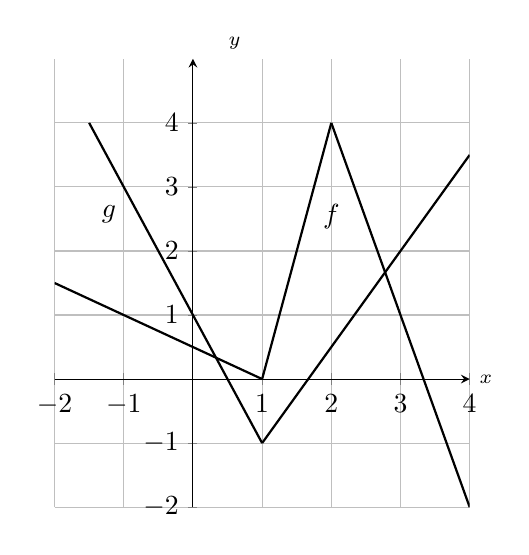
\begin{tikzpicture}
\begin{axis}[axis y line=middle,axis x line=middle, ymajorgrids=true, xmajorgrids=true, ymin=-2,ymax=5, xmin=-2,xmax=4, name=myplot, xscale=1/1.3, ytick={-2,-1,0,1,2,3,4}]
\addplot [draw={\colorone}, domain=-1.5:1,thick] {-2*x+1}; 
\addplot [draw={\colorone}, domain=1:4,thick] {1.5*x-2.5};
\addplot [draw={\colortwo}, domain=-2:1, thick] {-.5*x+.5};
\node[label={30:{$g$}}] at (axis cs:-1.6,2.2) {};
\addplot [draw={\colortwo}, domain=1:2, thick] {4*x-4};
\node[label={30:{$f$}}] at (axis cs:1.6,2.1) {};
\addplot [draw={\colortwo}, domain=2:4, thick] {-3*x+10};
\end{axis}
\node [right] at (myplot.right of origin) {\scriptsize $x$};
\node [above] at (myplot.above origin) {\scriptsize $y$};
\end{tikzpicture}}{The function f is the line segments connecting (-2,1.5) to (1,0) to (2,4) to (4,-2).  The function g is the line segments connecting (-1.5,4) to (1,-1) to (4,3.5).}\iflatexml\\\else\\*\fi
\begin{tabular}{ll}
(a) $(fg)'(-1)$  & (b) $(f/g)'(-1)$ \\
(c) $(fg)'(3)$ & (d) $(g/f)'(3)$
\end{tabular}}{(a) $-\frac72$ (b) $\frac1{18}$ (c) $-\frac92$ (d) $\frac{15}2$}

%\printreview

%\exercise{Given that $e^0=1$, approximate the value of $e^{0.1}$ using the tangent line to $f(x) = e^x$ at $x=0$.}{The tangent line to $f(x) = e^x$ at $x=0$ is $y=x+1$; thus $e^{0.1} \approx y(0.1) = 1.1$. }

%\exercise{Approximate the value of $(3.01)^4$ using the tangent line to $f(x) = x^4$ at $x=3$.}{The tangent line to $f(x) = x^4$ at $x=3$ is $y=108(x-3)+81$; thus $(3.01)^4 \approx y(3.01) = 108(.01)+81 = 82.08$. }
